\documentclass[a4paper,10pt]{article}
\usepackage{graphicx}
\usepackage[english]{babel}
\usepackage{subcaption}
\usepackage[latin1]{inputenc}
\usepackage[numbers]{natbib}
\usepackage{amsmath}
\bibliographystyle{unsrtnat}
\usepackage[top=1.5cm,bottom=2.5cm, left=2.5cm, right=2.5cm]{geometry}
\usepackage{siunitx}
\usepackage[parfill]{parskip}
\usepackage{multirow}
\setlength{\parskip}{1em}


\begin{document}

\begin{center}
    {\textbf{\Large{A.I. notes}}}\\
    {\large{Cooper}}
\end{center}

%%%%%%%%%% Main content %%%%%%%%%%
\section{Linear Regression}
\begin{itemize}
    \item \textbf{Hypothesis} function
        \begin{gather*}
            y = h(x) = \theta_0+\theta_1x\\
            y = h(x) = \pmb{\theta}\cdot\pmb{x}\\
        \end{gather*}

        \vspace*{-0.5cm}
    \item \textbf{Loss function}
        \begin{gather*}
            J(\theta_0. \theta_1) = \frac{1}{2}\frac{1}{m}\sum_{i=1}^{m}\Big(h(x^{(i)})-y_i\Big)^2 = \frac{1}{2}\frac{1}{m}\sum_{i=1}^{m}\Big(\theta_0+\theta_1x^{(i)}-y_i\Big)^2\\
            J(\theta_0,\theta_1,\dots,\theta_N) = \frac{1}{2}\frac{1}{m}\sum_{i=1}^{m}\Big(\theta_0+\sum_{k=1}^{N}\theta_kx_k^{(i)}-y_i\Big)^2
        \end{gather*}
    \item \textbf{Calculate the Gradient} gradient is the direction along which the loss function increases the most
        \begin{gather*}
            \nabla_\theta J_{(0)} = 
            \begin{pmatrix}
                \frac{\partial J}{\partial\theta_0} \\[0.4cm]
                \frac{\partial J}{\partial\theta_1} \\
            \end{pmatrix}_{(0)}
            \hspace*{0.7cm}
            \nabla_\theta J_{(0)} = 
            \begin{pmatrix}
                \frac{\partial J}{\partial\theta_0} \\[0.2cm]
                \frac{\partial J}{\partial\theta_1} \\[0.2cm]
                \vdots \\ 
                \frac{\partial J}{\partial\theta_N} \\
            \end{pmatrix}_{(0)}
        \end{gather*}

        \vspace*{-0.4cm}
    \item \textbf{Update}
        \begin{gather*}
            \pmb{\theta}_{(1)} = \pmb{\theta}_{(0)} - \alpha\nabla_\theta J_{(0)}\\
            \pmb{\theta}_{(n+1)} = \pmb{\theta}_n - \alpha\frac{1}{m}\mathbf{X}^T(\mathbf{X}\pmb{\theta}_n-\pmb{y})
        \end{gather*}
    \item \textbf{Repeat}.
        \begin{gather*}
            \pmb{\theta}_{(n+1)} = \pmb{\theta}_{(n)} - \alpha\nabla_\theta J_{n}\hspace*{0.5cm}n = 0,1,2,\dots\\
            \text{Stop if}\hspace*{0.3cm}\left| J_{(n+1)}-J_n \right|\leq\text{tol}\hspace*{0.5cm}\text{or}\hspace*{0.3cm}n+1\geq\text{ max}
        \end{gather*}
\end{itemize}

\subsection{Regularisation}
A good machine learning model should have a good \textit{bias-variance trade-off}. This can be achieved by minimising the generalisation error, which is the sum of the squared bias and the variance. 
\begin{gather*}
    J(\theta_0. \theta_1) = \frac{1}{2}\frac{1}{m}\sum_{i=1}^{m}\Big(h(x^{(i)})-y_i\Big)^2 + \lambda\sum_{j=1}^{N}\theta_j^2
\end{gather*}
If $\lambda$ is small, large values of $\sum_{j=1}^{N}\theta_j^2$ are allowed, meaning that the model contains too many parameters, thus it can \textbf{overfit}. If $\lambda$ is large, only small values of $\sum_{j=1}^{N}\theta_j^2$ are allowed. This means that the training will reduce the number of parameters, this it might underfit. 

\section{Logistic Regression}
\begin{itemize}
    \item \textbf{Hypothesis function}, models the probability that a given set of features belongs
    to class
        \begin{gather*}
            h(\mathbf{x}) = \sigma(\mathbf{\theta\cdot x}) = \frac{1}{1+exp(-\theta\cdot x)}
        \end{gather*}
    \item \textbf{Loss function} (cross-entropy), entropy measures uncertainty on the possible values of a prediction
        \begin{gather*}
            J(\theta) = -\frac{1}{m}\sum_{i=1}^{m}\Big\{y_i ln\Big[h(x^{(i)})\Big] + (1-y_i)ln\Big[1-h(x^{(i)})\Big]\Big\}
        \end{gather*}
    \item \textbf{Gradient descent} for logistic Regression:\par
    Choose a starting point $\Rightarrow$ Calculate hte gradient $\Rightarrow$ Update and repeat. 
    \item If encounter \textbf{multi-class}, perform the same as many times as the number of categories of logistic regressions, each of which splits the data into two classes. End up with the same number of Hypothesis functions, select the highest probability.
    \item Metrics for classification 
        \begin{table}[hbt]
            \centering
            \begin{tabular}{lcccl}
            \cline{3-4}
                                & \multicolumn{1}{l|}{}           & \multicolumn{2}{c|}{\textbf{Ground Truth}}                               &  \\ \cline{3-4}
                                & \multicolumn{1}{c|}{}           & \multicolumn{1}{c|}{\textbf{1}}     & \multicolumn{1}{c|}{\textbf{0}}    &  \\ \cline{1-4}
            \multicolumn{1}{|c|}{\multirow{2}{*}{\textbf{\begin{tabular}[c]{@{}c@{}}Model\\ Prediction\end{tabular}}}} &
            \multicolumn{1}{c|}{\textbf{1}} &
            \multicolumn{1}{c|}{True Positive} &
            \multicolumn{1}{c|}{False Positive} &
            \multicolumn{1}{c}{\textbf{Precision}} \\ \cline{2-4}
            \multicolumn{1}{|c|}{} & \multicolumn{1}{c|}{\textbf{0}} & \multicolumn{1}{c|}{False Negative} & \multicolumn{1}{c|}{True Negative} &  \\ \cline{1-4}
                                & \multicolumn{1}{l}{}            & \textbf{Recall}                     & \multicolumn{1}{l}{}               & 
            \end{tabular}
        \end{table}
\end{itemize}

\subsection{Supporting Vector Machines (SVMs)}
In SVMs, we want to compute the optimal linear decision boundary, which is the \textbf{hyperplane} with the largest margin between the two classes.
\begin{itemize}
    \item Support hyperplanes (optimal hyperplane between two points)
    \begin{gather*}
        \mathbf{w}\cdot\mathbf{x} + b = 1\\
        \mathbf{w}\cdot\mathbf{x} + b = -1\\
    \end{gather*}

    \vspace*{-0.8cm}
    How is the hyperplane with largest margin oriented can be found by solving an optimisation problem
    \begin{gather*}
        \text{Find }\mathbf{w},b\text{ such that }\frac{2}{\lVert w \rVert}\text{ is maximum}\\
        \text{or }\min\limits_{(w,b)}\frac{1}{2}{\lVert w \rVert}^2\hspace*{0.3cm}\text{subject to}\hspace*{0.3cm}y_i(\mathbf{w}\cdot\mathbf{x}^{(i)}+b)\geq1\hspace*{0.3cm}i = 1,2,\dots,m
    \end{gather*}
\end{itemize}

\subsubsection{Rgularisation}
if the data is not linearly separable, we need to introduce regularisation to allow some misclassified data points by introducing a slack variable $\varepsilon_i>0$ such that: (i) $\varepsilon_i=0$ for correctly classified (ii) $\varepsilon_i=\left| y_i-f(\mathbf{x}^{(i)})\right|$ otherwise. 
\begin{gather*}
    \min\limits_{(w,b,\varepsilon)}\frac{1}{2}{\lVert w \rVert}^2+C\sum_{i}^{m}\varepsilon_i\hspace*{0.3cm}\text{subject to}\hspace*{0.3cm}y_i(\mathbf{w}\cdot\mathbf{x}^{(i)}+b)\geq1-\varepsilon_i\hspace*{0.3cm}\varepsilon_i\geq0\\
    \text{small C - soft (wide margin)}\hspace*{0.4cm}C\rightarrow\infty\text{ - hard margin}
\end{gather*}

\subsubsection{Kernel Trick}
For nonlinearly separable data, one option is to enrich the data with nonlinearities. This can be achieved by mapping the data into a nonlinear higher-dimensional space, $\mathbf{x}\rightarrow\mathbf{\phi(x)}$, where $\mathbf{\phi}$ is a nonlinear map, for example, a polynomial $(x_1^{(i)},x_2^{(i)})\rightarrow(x_1^{(i)},x_2^{(i)},x_1^{(i)2}+x_2^{(i)2})$. Intuitively, by adding dimensions in the feature space, it is more likely that the data becomes linearly separated.\par 

Kernel Trick decomposes the weight vector in the transformed feature space
\begin{gather*}
    \mathbf{w} = \sum_{j=1}^{m}\beta_j\pmb{\phi}(\pmb{x}^{(j)})
\end{gather*}
where $\beta_j$ become the new weights to find. In other words, we express the weight vector with coordinates defined in the transformed feature space.
\begin{gather*}
    f(\pmb{x}^{(i)}) = \sum_{j=1}^{m}\beta_j\pmb{\phi}(\pmb{x}^{(j)})\cdot\pmb{\phi}(\pmb{x}^{(i)})+b 
\end{gather*}
we resort to a theorem of functional analysis, which ensures that there exists a function, $K$, such that
\begin{gather*}
    K(\pmb{x}^{(j)}\cdot\pmb{x}^{(i)}) = \pmb{\phi}(\pmb{x}^{(j)})\cdot\pmb{\phi}(\pmb{x}^(i))
\end{gather*}
where $K$ is the \textit{kernel}. $K$ suggested that we DO NOT need to increase the dimension of the feature space to include nonlinearities, we only need to apply the kernel to inner products in the original feature space. essentially finding optimal separating hyperplane without calculating anything about $\pmb{\phi(x^{(i)})}$.





\section{Feedforward Neural Network}
\textit{Neural Network generalise the principle of linearly combining simple nonlinear functions}
\begin{gather*}
    y\approx h(x:\theta)
\end{gather*}
function that maps input data "x" to output "y", with the function parameters represented by "$\theta$".

\begin{figure}[ht]
    \centering
    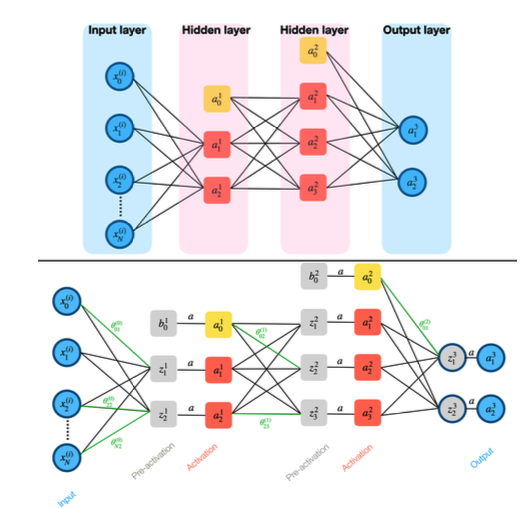
\includegraphics[width =0.5\textwidth]{FNN.png}
\end{figure}

\subsection{Mathematical expression}
\begin{itemize}
    \item Input layer $\rightarrow$ First hidden layer
        \begin{gather*}
            x  = 
            \begin{pmatrix}
                x_{1} \\
                x_{2} \\
                \vdots \\
                x_{m} \\
            \end{pmatrix}
            \Rightarrow\hspace*{0.4cm}\theta^{(0)} = 
            \begin{pmatrix}
                \theta_{0,1}^{(0)} & \theta_{0,2}^{(0)}  \\
                \theta_{1,1}^{(0)} & \theta_{1,2}^{(0)}  \\
                \vdots \\
                \theta_{N,1}^{(0)} & \theta_{N,2}^{(0)}  \\
              \end{pmatrix}
              ,\hspace*{0.3cm}
              z^1 = 
              \begin{pmatrix}
                b_0^1 \\
                \theta^{(0)T}x \\
              \end{pmatrix}
              ,\hspace*{0.3cm}
              a^1 = a\{z^1\} 
        \end{gather*}
    where $z$ is the \textit{pre-activation}
    \item Second hidden layer 
        \begin{gather*}
        \theta^{(1)} =
            \begin{pmatrix}
                \theta_{0,1}^{(1)} & \theta_{0,2}^{(1)} & \theta_{0,3}^{(1)}  \\
                \theta_{1,1}^{(1)} & \theta_{1,2}^{(1)} & \theta_{1,3}^{(1)} \\
                \theta_{2,1}^{(1)} & \theta_{2,2}^{(1)} & \theta_{2,3}^{(1)} \\
            \end{pmatrix}
            ,\hspace*{0.3cm}
            z^2 = 
            \begin{pmatrix}
                b_0^2 \\
                \theta^{(2)T}a^1 \\
            \end{pmatrix}
            ,\hspace*{0.3cm}
            a^2 = a\{z^2\} 
        \end{gather*}
    \item Output layer 
        \begin{gather*}
            \theta^{(1)} =
                \begin{pmatrix}
                    \theta_{0,1}^{(2)} & \theta_{0,2}^{(2)} \\
                    \theta_{1,1}^{(2)} & \theta_{1,2}^{(2)} \\
                    \theta_{2,1}^{(2)} & \theta_{2,2}^{(2)} \\
                    \theta_{3,1}^{(2)} & \theta_{3,2}^{(2)} \\
                \end{pmatrix}
                ,\hspace*{0.3cm}
                z^3 = \theta^{(2)T}a^2
                ,\hspace*{0.3cm}
                h = a^3 = a\{z^3\} 
            \end{gather*}
            Or in generalised from
            \begin{gather*}
                a^{L+1} = a\{\theta^{(L)T}a^L\}
            \end{gather*}
\end{itemize}

\subsection{Number of parameters}
\begin{gather*}
    \begin{split}
        \text{n. of parameters} &= \underbrace{(s_0+1)\times s_1}_{(N+1)\times 2} + \underbrace{(s_1+1)\times s_2}_{3\times 3} + \underbrace{(s_2+1)\times s_3}_{4\times 2} = (N+1)\times 2+17\\
        & = \sum_{i=0}^{L}(s_i+1)\times s_{i+1}
    \end{split}
\end{gather*}

\subsection{Training}
Training dataset (60-8-\%), Validation (10-20\%), and test (10-20\%)\par 

Initialise $\Rightarrow$ Forward propagation $\Rightarrow$ Backpropagation $\Rightarrow$ Update $\Rightarrow$ Repeat until convergence



\section{Convolution Neural Network}
Drawbacks from feed-forward neural networks 
\begin{itemize}
    \item textit{fully connected} layers not suitable for images: contains too many parameters  
    \item need to \textit{flatten} 2D data into 1D array --- losing spatial information. 
\end{itemize}

Generic process
\begin{itemize}
    \item input $\rightarrow$ filter (convolutional layer)$\rightarrow$ pooling layer $\rightarrow$ (repeat) $\rightarrow$ flatten $\rightarrow$ fully-connected layer
    \item Numbers of neurons in a convolutional layer
        \begin{gather*}
            N_d = \frac{W_d-F_d+2P_d}{S_d}+1
        \end{gather*}
    where $N_d$ is the number of neurons, $W$ is the width of the input channel, $F$ is the width of the filter, $P$ is the width of the pooling, and $S$ is the Stride number. 
    \item Number of parameter in convolution layer $l$
        \begin{gather*}
            l = (F_x\times F_y\times \text{n. channels} + 1 \text{ bias})\times K
        \end{gather*}
    where $K$ is the number of filters (also =number of feature maps)
\end{itemize}



\section{Sequence Modelling}
When both the data and its order contain information to perform the task, the points in the dataset are dependent on the position of other points in the dataset, e.g., speech recognition, DNA, time series. We lose key information if we shuffle the data.

\subsection{Sequence modelling with feedforward neural network}
Consider time as \textbf{feature (inputs)}, and the physical variable as \textbf{label}, may be OK for short time series, but generally not a good approach due to:
\begin{itemize}
    \item do not learn correlation as opposed to dynamical system having temporal correlations, and patterns. 
    \item large number of parameters
    \item needs the inputs of a fixed size. 
\end{itemize}

\subsection{Recurrent cell}
Store the previous time-step and feed it to the next time step as the hidden state.
\vspace*{0.3cm}
\begin{gather*}
    a^{<N>} = a(\theta_a^{<N-1>}+\theta x^{<N>}+b)\\
    h^{<N>} = \theta_ha^{<N>}+b_h
\end{gather*}

\vspace*{-0.3cm}
\begin{figure}[ht]
    \centering
    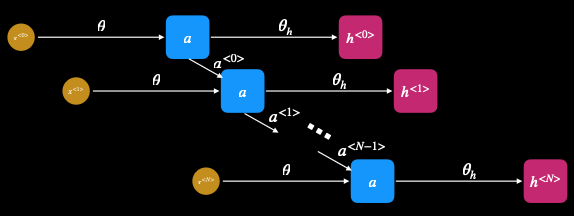
\includegraphics[width =0.6\textwidth]{RC.png}
\end{figure}

\begin{itemize}
    \item The weights and biases are shared across the time-step
    \item \textbf{time is not a feature}
    \item the loss function is a sum of the loss functions of every time step by applying chain rule across different time steps. 
        \begin{gather*}
            J = \sum_{i=0}^{N}J^{<N>}\\
            \frac{\partial J}{\partial a^{<i>}} = \frac{\partial J}{\partial a^{<N>}}\frac{\partial a^{<N>}}{\partial a^{<N-1>}}\dots\frac{\partial a^{<i+1>}}{\partial a^{<i>}} = \frac{\partial J}{\partial a^{<N>}}\underbrace{\theta_a\theta_a\dots\theta_a}_{N-i\text{ times}} = \frac{\partial J}{\partial a^{<N>}}\theta_a^{N-1}
        \end{gather*}
    \item Unstable gradient occurs from above equation, when $\theta_a$ is small, the gradient will become smaller and leads to \textbf{vanishing gradient} problem,  make it difficult for the network to remember information from previous time steps. This can be solved by using ReLU activation functions due to its unbounded positive range. 
    \item If $\theta_a$ is large, this leads to exploding gradient, which can be solved by clip (rescale) the gradient
    \item Recurrent neural network are not ideal for learning temporal correlations in long time series due to short-term memory. 
\end{itemize}

\subsection{Long-short time memory units LSTMs}
Introducing a \textit{cell state C} to convey (store) information from the far past -- long term memory, with the combination of the same short-memory past. 
\begin{itemize}
    \item Consists of three gates to control the status of the states (forget, input, output). Each gate is controlled by a \textbf{sigmoid} activation function, due to the extreme nature of being either 1 or 0.
    \item \textbf{Forget gate.} This determines what percentage of the Long-term memory is remembered. 
    \item \textbf{Candidate state} combines the shor-term memory and the input to create a \textbf{potential long-term memory} $g$. By using \textbf{tanh} to restrain the data in the range of -1 to 1. 
    \item \textbf{Input gate} determines what percentage of the potential long-term memory is added to the long term memory $C$.
    \item \textbf{Output gate} calculates the potential long term memory from the cell state using a tanh function. Then, a sigmoid function is also used to determine what percentage of this potential long term memory is pass on as an output of the LSTM unit. 
\end{itemize}

\subsection{Gated recurrent units GRUs}
\begin{itemize}
    \item got rid of the cell state, and stored both long and short term memory in the \textbf{hidden state} and consists of 2 gates only.
    \item \textbf{Update gate} controls both the \textit{input} and \textit{forget} gate in determining what to forget and what to add on. 
    \item \textbf{Reset gate} decides how much past information to forget. 
    \item \textbf{Candidate state} contains past information.
    \item GRUs are simpler and with less parameters, making them easier to train than LSTMs
\end{itemize}

\vspace*{-0.3cm}
\begin{figure}[ht]
    \centering
    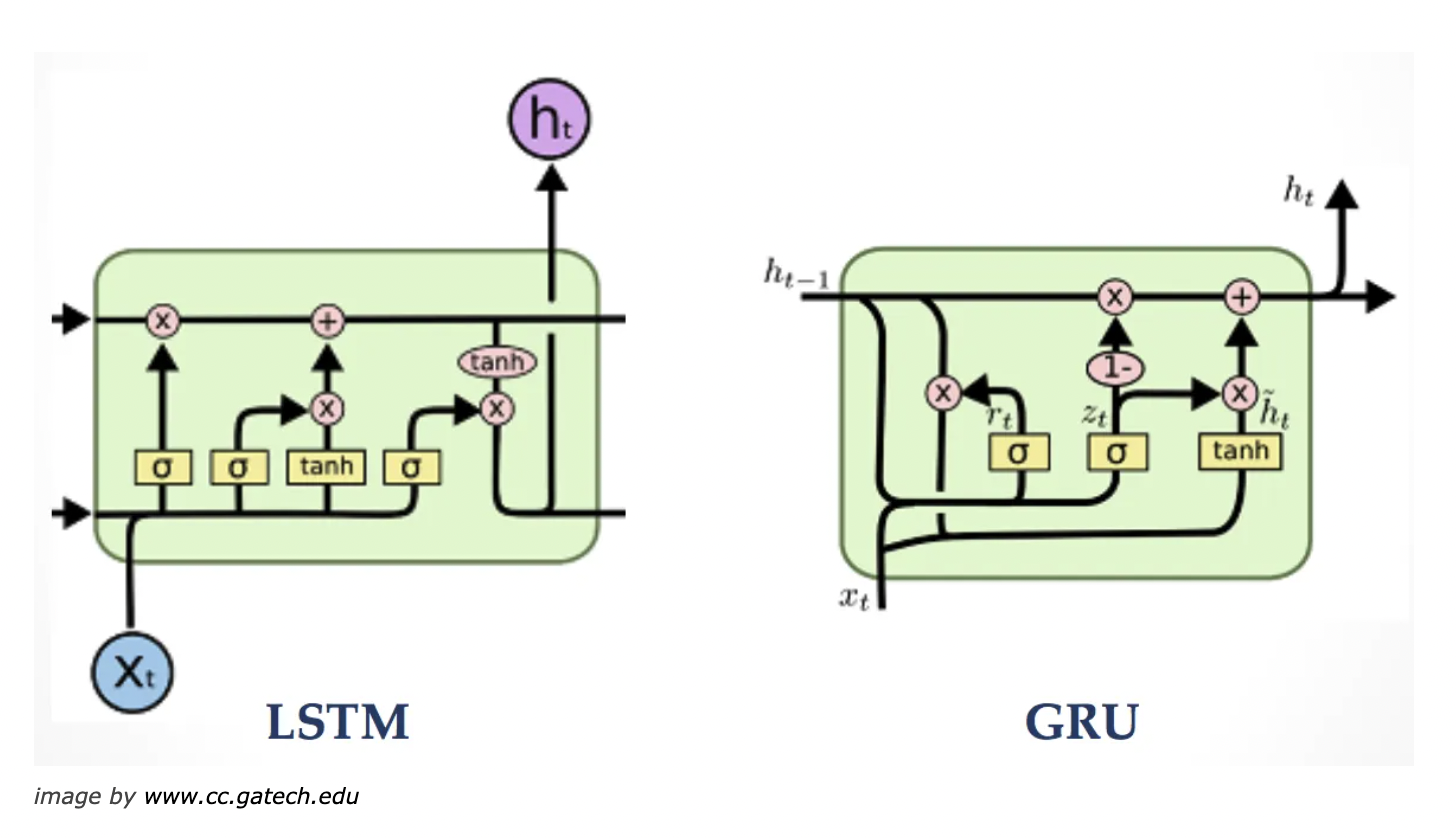
\includegraphics[width =0.7\textwidth]{LSTM_GRU.png}
\end{figure}


\section{Unsupervised Learning}
methods that do not require labelled dataset. 

%%%%%%%%%% %%%%%%%%%%



\end{document}
 